\documentclass[letter,12pt,dissertation]{OUdissertation5} %for Ph.D. disseration style
%\documentclass[letter,12pt,thesis]{OUdissertation5} %for M.S. thesis style
\usepackage{graphicx} %allows .eps and .epsi graphics to be inserted
\usepackage{epic} %allows use of latex graphics
\usepackage{eepic} %allows use of latex graphics
\usepackage{amssymb}
\usepackage{amsfonts}
\usepackage{psfrag}
\usepackage{float}
\usepackage{bar}
% Brian added this on July 15 2006 from suggestion of Di Jin:
\usepackage[centerfoot]{pageno}

%\usepackage{harvard} %use with agsm.bst, see near end
%\newcommand{\citet}[1]{\citeasnoun{#1}} %use this with harvard 
%\newcommand{\citep}[1]{\cite{#1}} %use this with harvard 

\usepackage{natbib} %with amermeteorsoc.bst
%% For AMS,citations should be of the form ``author year''  not ``author, year'':
\bibpunct{(}{)}{;}{a}{}{,}

\newcommand{\be}{\begin{equation}} %these definitions save typing
\newcommand{\ee}{\end{equation}}
\newcommand{\bea}{\begin{eqnarray}}
\newcommand{\eea}{\end{eqnarray}}
\newcommand{\pd}[2]{\frac{\partial#1}{\partial#2}}
\newcommand{\pdd}[3]{\frac{\partial^{2}#1}{\partial#2 \partial#3}}


\begin{document}
\title{ USING \LaTeX\  TO WRITE \\ A DISSERTATION AT O.U.}
\author{BRIAN FIEDLER}
\depositdate{1998}
\majorfield{SCHOOL OF METEOROLOGY}
\memberone{Prof. Albert Einstein}
\membertwo{Prof. Enrico Fermi}
\memberthree{Prof. Alfred E. Newman}
%next two members are used in dissertation
\memberfour{Dr. Homer Simpson}
\memberfive{Dr. Strangelove}
%another member is possible, but you must hack OUdissertation.cls
\membersix{Dr. Spock}
%%%%
\begin{preface}
%\prefacesection{Dedication} %Dedication must be without a pagenumber, see end of this file.
%This dissertation is dedicated to Donald Knuth and Linus Torvalds.
\prefacesectionX{Dedication}
This dissertation is dedicated to Donald Knuth and Linus Torvalds.

A dedication page is optional in the OU dissertation.  
This section is not allowed to have a printed pagenumber, nor is it allowed to
increment the page number counter. This is why we use the hacked \verb+\prefacesectionX+ for
the Dedication, rather \verb+\prefacesection+.
\prefacesection{Acknowledgements}
I would like to thank Prof. Einstein and Prof. Fermi
for their expert advice  and  patience.  Their sacrifice
was enormous, considering the fact that I got a D in
freshman physics --- and I never really got much better after that.
%must leave a blank line next to avoid bug:

\tableofcontents
\listoftables
\listoffigures
\prefacesection{Abstract}
 In 1998, I hacked the \texttt{OUdisseration.cls} file from the 
{\tt USCthesis.cls} file that I grabbed from the web.
As of April 21, 2009, this ``dissertation'' uses the \texttt{OUdisseration5.cls} to define the
document class.
The comments inside \texttt{OUdissertation5.cls} describe the changes.
(You may see a bug here with the text extending past the margin.)
 
I put this example ``dissertation'' together for the benefit of
the students at the University of Oklahoma, who can use it as a 
template for their own work.   Depending on the demand of the users,
maybe someday I will clean this up.  {\it Caveat user}.
\end{preface}
\chapter{Introduction}
\label{intro}
\citet{Daley} and \citet{GhilMal} refer 
to this problem as the ``data assimilation'' problem.  But I can 
write this sentence a different way:  Consequently, this problem 
is referred to as the ``data assimilation'' problem 
\citep{Daley,GhilMal}.  I will let the text run on here a bit so that
a big reference list will be generated.

Formally, let $c$ be a control vector of size $m$ and $S$ denote the 
feasible region for the control vector.  For any $c$ in $S$, let 
$J(c)$ denote the weighted sum of the squared difference between the 
observation and the solution of the model corresponding to the control 
vector $c$.  Except in trivial cases the explicit form of $J$ as a 
function of $c$ is not known.  It is to be emphasized that there are 
other possible choices for the $J$ function.  One may be interested 
only in the state of the model at a given time instant, say $t = 
\Delta$.  Whatever be the nature and type of the $J$ function, 
mathematically, the data assimilation problem can be stated as follows 
: find a $c^{*}$ in $S$ such that $J(c^{*})$ is a minimum, that is, we 
are lead to an optimization problem under the dynamical constraints of 
the model equations.  Since $J$ is a ``smooth'' function, one method 
for finding $c^{*}$ is to use one of the many variants of the 
classical gradient method.  This is however, more easily said than 
done.  The difficulty primarily stems from the fact that $J$ is not 
known explicitly.  A now popular method for finding the gradient of 
$J$ is called the ``adjoint'' method \citep{GhilMal,ThackLong}.  A 
summary of data assimilation using the adjoint method is shown in Fig.  
\ref{flowchart} and described below:


Considerable success has been reported in the literature in the use of 
adjoint method for finding $c^{*}$  
\citep{Luenberger,SunFlick,Wolfsberg}.  The success of this combination is largely 
dependent on the properties of the $J$ function.  This approach can 
succeed only if $J$ is unimodal in $S$.  It turns out that the 
modality of $J$ critically depends on the model dynamics.  It is now 
known that the nonlinearity in the model dynamics induces 
multimodality in the $J$ function \citep{Li,Chung}.

There are at least two factors affecting the rate of convergence of 
the iterates leading to the optimum value of the $J$ function.  First,
is the number and distribution of the observations.  There is a minimum 
number of observations required from an algorithmic viewpoint, but 
satisfaction of this requirement is insufficient to guarantee a solution.
The distribution of these data (in space and time), in concert wtih 
the dynamics, dictates the existence of a solution.  Second, is the shape 
of the $J$ function.  Judicious choice of scaling can remove 
eccentricities in the $J$-field.  It is thus imperative 
to understand the role of these two factors affecting the iterates.

The effect of the number and distribution of observations on the 
quality of the 
iterates are often examined using controlled experiments which have come 
to be known as the ``twin'' experiments.  In this, a point in the 
feasible region for the control vector is first chosen and then the 
model solution is calculated for this value of the 
control vector .  Then observations (including known error) are generated from 
the model solution by adding noise with known characteristics.  
By computing the optimal estimate of the control vector for different 
sets of observations, we can develop a better understanding 
of the dependence of the optimal estimate on the number, distribution
 and accuracy of observations.

As for the shape of the $J$ function, since it is not known 
explicitly, we must be contented with the analysis of the 
properties of $J$ around the local minima.  This is often done 
by approximating $J$ around the optimum $c^{*}$ using a quadratic form 
such as \be J(c) = \frac{1}{2}c^{t} H c + p^{t} c + q , \ee where $H$ 
is the Hessian matrix which is a symmetric matrix of the second 
derivatives of $J$ with respect to $c$, \be p = \left( p_{1} , p_{2} , 
p_{3} , p_{4} , ...  , p_{n}\right)^{t} \ee is a vector and $q$ is a 
constant.  By analyzing the eigenvalues of $H$, we can draw inferences 
on the shape of $J$ in the vicinity of $c^{*}$ \citep{Thacker}.  For 
example, if one of the eigenvalues of $H$ is very small, then the 
contours or the level curves of $J$ for the valley around $c^{*}$ are 
elongated ellipses.  This would imply that the iterative process of 
locating the minimum would converge slowly and with difficulty.

In this dissertation, one aim is to apply the adjoint method to the 
mixed layer model \citep{Ball,Lilly}.  This model is used to predict 
the return flow of the warm, humid air from the Gulf of Mexico into 
the coastal plains during the winter months.  The mixed layer model 
has a small number of unknown variables/parameters.  Athough small, the model
is nonlinear and thus presents difficulties in dynamical optimization.
With the experience gained, we wanted to analyze the computational aspects of 
data assimilation.  This brought us to the shallow water equations 
\citep{Pedlosky}, which has a larger number of variables in the
discrete model.  We are interested in solving some of the 
computational aspects of this model that are relevant to data 
assimilation.  Since the solution of the forward model and the adjoint 
take a good fraction of the efforts, we turned our attention to 
parallel methods for solving this class of equations.

The shallow water model is discretized first using the Euler scheme.
  But due to its instability, we also examined
 the solution using a stable 
leapfrog scheme.  Both types of discretization resulted 
in a block bi-diagonal system of equations for the forward model and 
the adjoint model.  We are interested in examining the comparative 
analysis of four vector/parallel algorithms in solving this system of 
equations.
These four vector/parallel algorithms belong to a class of direct 
parallel methods.  The first algorithm is also known as the ``divide and 
conquer'' method \citep{Varahan}.  The second algorithm is a variation
of the divide and conquer method \citep
{Varahan,Conn,MeyerPod87,Vandervorst,MeyerPod89}.  The third 
algorithm is
known as the partition algorithm \citep{Vandervorst89}. The fourth 
algorithm is the
cyclic reduction method \citep{Varahan}. A comparison of these four 
vector/parallel algorithms is done on the CrayJ90 in scalar mode and 
using 1,2,4 and 8 vector processors.

 This dissertation is organized as follows.  A description of the use
 of encapsulated postscript files is presented in Chapter 
 \ref{eps_pdf_examp}.  One way to present bargraphs is shown in
 model equations are described in Section \ref{bargraph}.  Some example
 tables are shown in Section \ref{table}.  





\chapter{Mostly {\tt .eps and .pdf} examples}
\label{eps_pdf_examp}

This chapter shows how encapsulated postscript figures can be included in
the document.  In particular, we wish to show how raw {\tt .eps} and {\tt .pdf}
files can annotated and labeled to make them of ``publication quality''.

\section{A few easy equations and a picture}
\begin{figure}[H]
\setlength{\unitlength}{1mm}
\begin{center}
\setlength{\unitlength}{1mm}
\begin{picture}(100,60)
\dashline{3}(0,45)(100,45)
\dashline{3}(0,42)(100,42)
\drawline(0,5)(100,5)
\put(10,55){\vector(0,-1){50}}
\put(11,50){$\frac{S_{0}}{4}$}
\put(12,5){\vector(0,1){30}}
\put(13,35){$\frac{S_{0}}{4} \alpha_{p}$}
\put(45,5){\vector(0,1){30}}
\put(47,15){$\sigma T^{4}_{s}$}
\put(45,45){\vector(0,1){10}}
\put(47,50){$(1-\epsilon )\sigma T^{4}_{s}$}
\put(80,45){\vector(0,1){10}}
\put(82,47){$\epsilon \sigma T^{4}_{a}$}
\put(80,42){\vector(0,-1){10}}
\put(82,38){$\epsilon \sigma T^{4}_{a}$}
\end{picture} 
 %this works with latex, but not pdflatex
%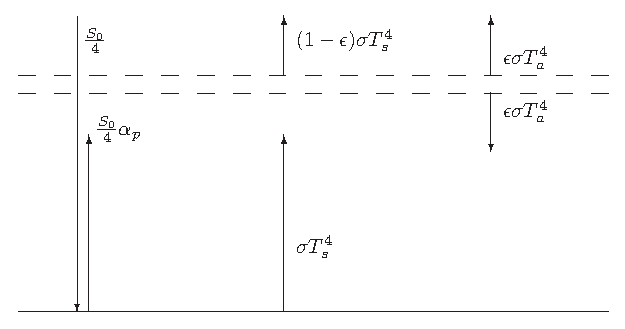
\includegraphics[width=4in]{greenhouse} %uses .pdf in pdflatex, and .eps in latex 
\caption[Radiative equilibrium]{Radiative equilibrium with a ``greenhouse effect''.  This
picture was drawn using \LaTeX\ {\tt epic} commands in the so-called {\em picture
environment}. With {\tt pdflatex}, the horizontal lines will be missing. 
{\tt pdfprob.tar.gz} shows the more complicated procedure to include epic
figures with {\tt pdflatex}.} 
\label{greenhouse}
\end{center}
\end{figure}
A radiative balance at the surface requires that: 
\be
\frac{S_{0}}{4} (1-\alpha_{p})+
\epsilon \sigma T^{4}_{A} 
= \sigma T^{4}_{s}.
\label{surbal}
\ee
Radiative equilibrium of the putative ``atmosphere'' in Figure \ref{greenhouse} requires that:
\be
\epsilon \sigma T^{4}_{s} 
= 2\epsilon \sigma T^{4}_{s}. 
\label{atmosbal}
\ee
We use (\ref{atmosbal}) to eliminate $T_{A}$ from (\ref{surbal}),
which gives:
\be
\frac{S_{0}}{4} (1-\alpha_{p})+
\frac{1}{2}\epsilon \sigma T^{4}_{s} 
= \sigma T^{4}_{s}. 
\label{equi}
\ee
or
\be
T_{s}=\sqrt[4]{
\frac{S_{0}(1-\alpha_{p})}{4\sigma (1-\frac{\epsilon}{2})}}
\ee
\section{Simple inclusion of {\tt .eps} or {\tt .pdf} graphics}
\begin{figure}[H]
\begin{center}
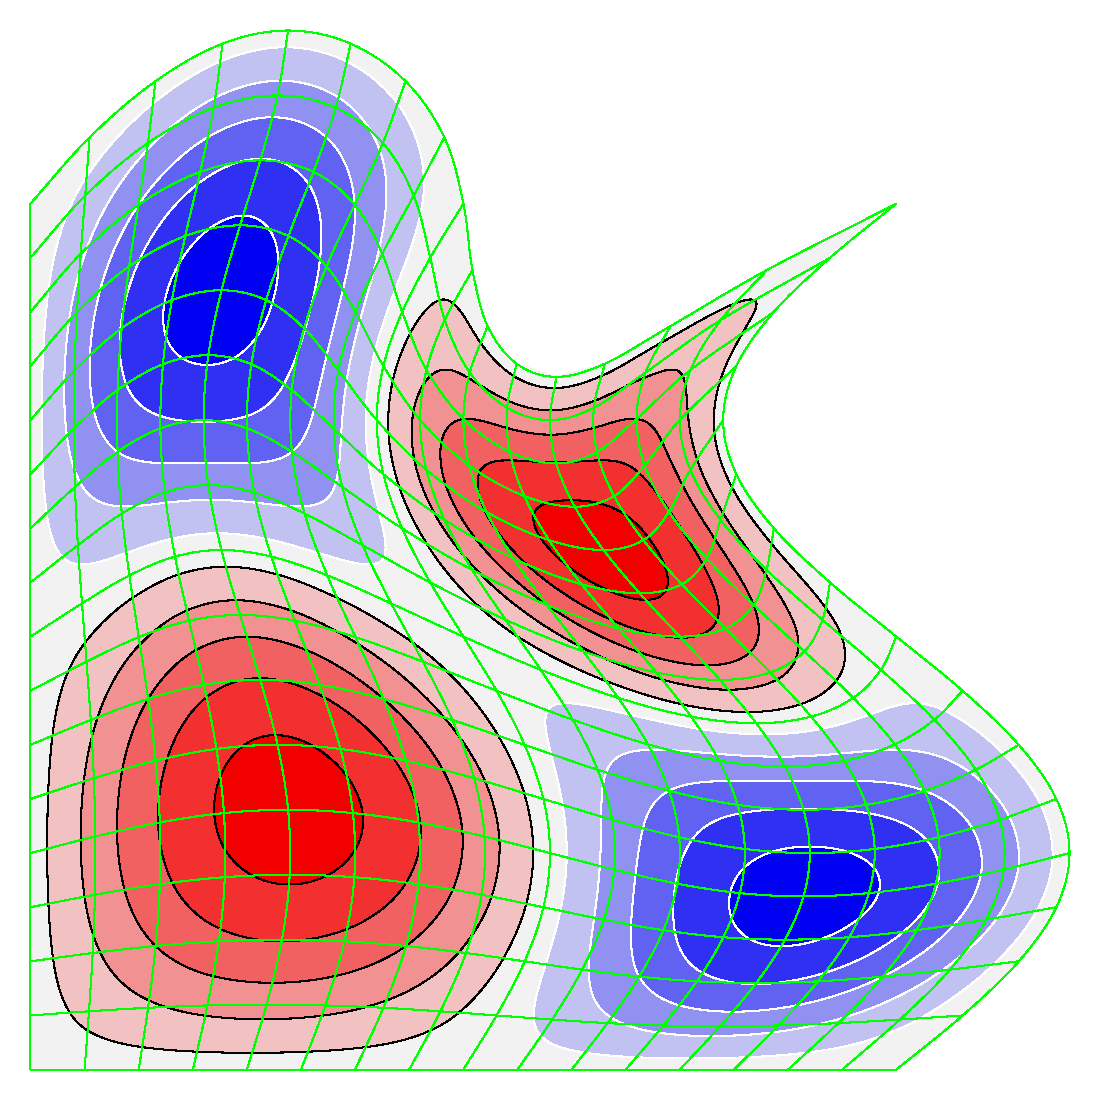
\includegraphics[width=3in]{squash2} 
\end{center}
\caption[Melted figure]{This is what happens when you leave your figure in a hot car
during July.}
\end{figure}
\begin{figure}[H]
\begin{center}
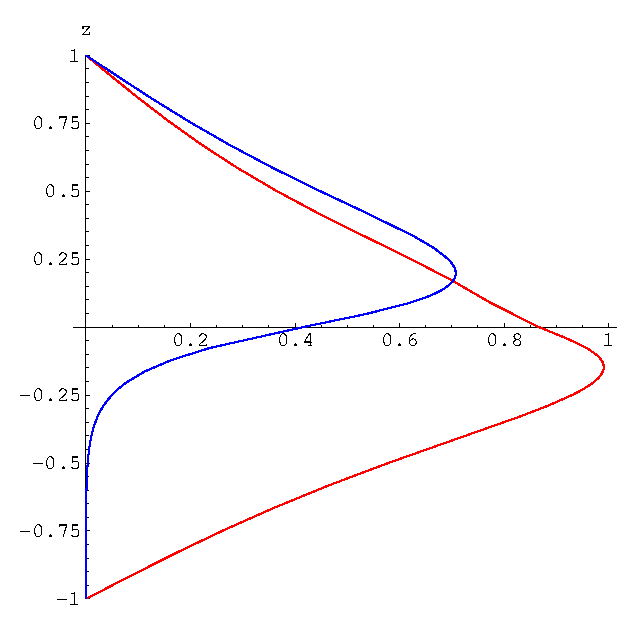
\includegraphics[width=3in]{hitplot}
\end{center}
\caption[Raw {\tt .eps}]{Raw {\tt .eps} from {\bf Mathematica}.}
\end{figure}
%%%%
\section{{\tt .eps or .pdf}, annotated }
\begin{figure}[H]
\setlength{\unitlength}{1in}
\begin{center}
\begin{picture}(3,3)(0,0)
\put(.2,.2){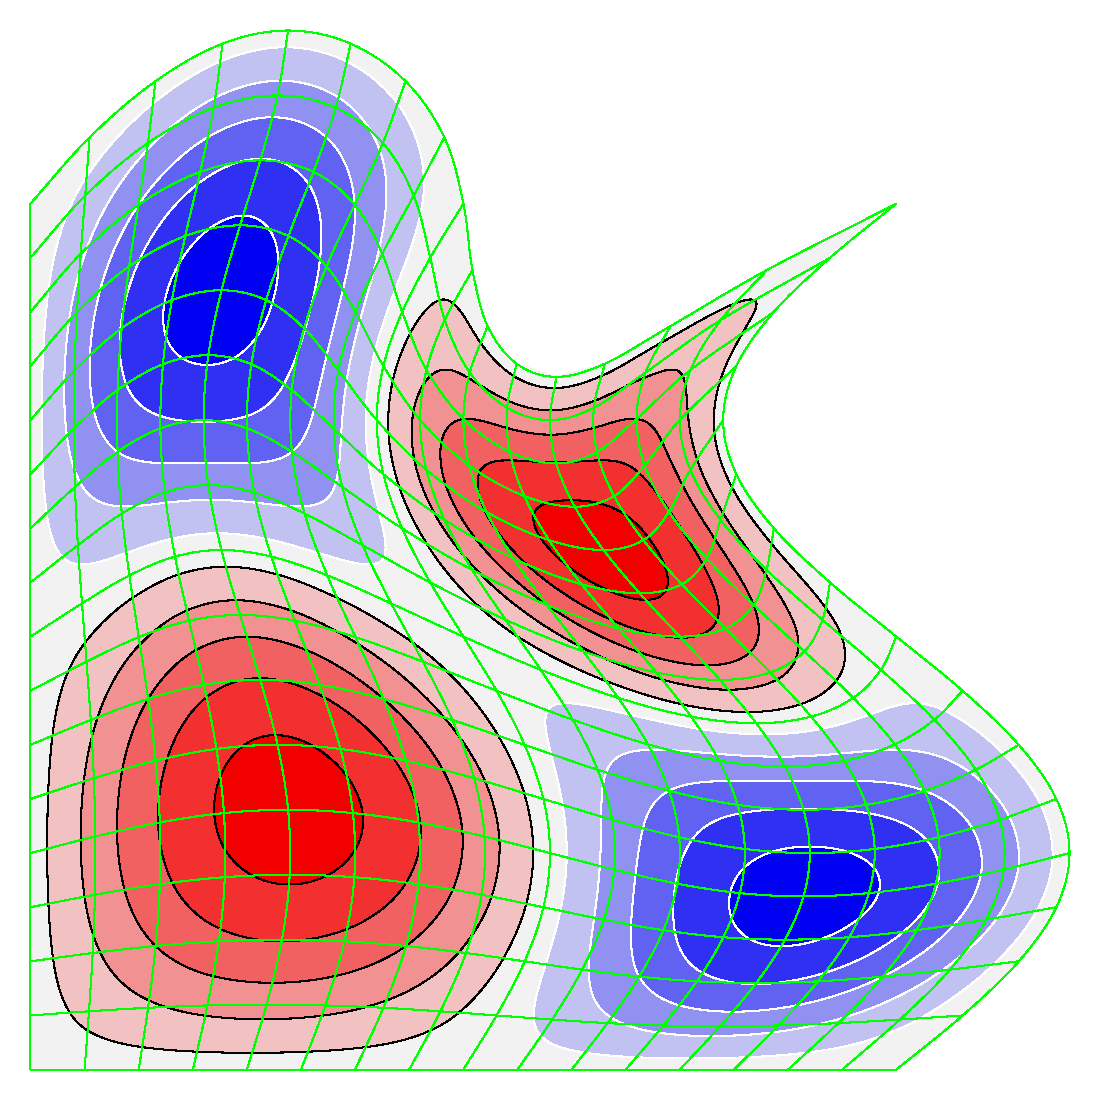
\includegraphics[width=2.6in]{squash2}}
\put(1.7,.1){\vector( 1,0){1.1}}
\put(1.3,.1){\vector(-1,0){1.1}}
\put(1.5,.1){\makebox(0,0)[c]{$\int x dx$}}
\put(.1,1.7){\vector( 0,1){1.1}}
\put(.1,1.3){\vector(0,-1){1.1}}
\put(.1,1.5){\makebox(0,0)[c]{$\frac{y}{x}$}}
\put(1.4,2.2){$E=mc^2$}
\end{picture}
\end{center}
\caption[Annotated melted figure]{The melted figure with annotations.
Wonderful! All of the epic commands here work in both {\tt latex} and {\tt pdflatex},
in Fig. \ref{greenhouse} some did 
did not in {\tt latex}.  This is may favorite way to put labels on my figures.}
\end{figure}
%%%%%%%%%
\section{Using the {\tt psfrag} system with .eps}
\begin{figure}[H]
\begin{center}
\psfrag{z}{\Large $\zeta$}
\setlength{\unitlength}{1in}
\begin{picture}(2.5,2.5)(0,0)
\put(0,0){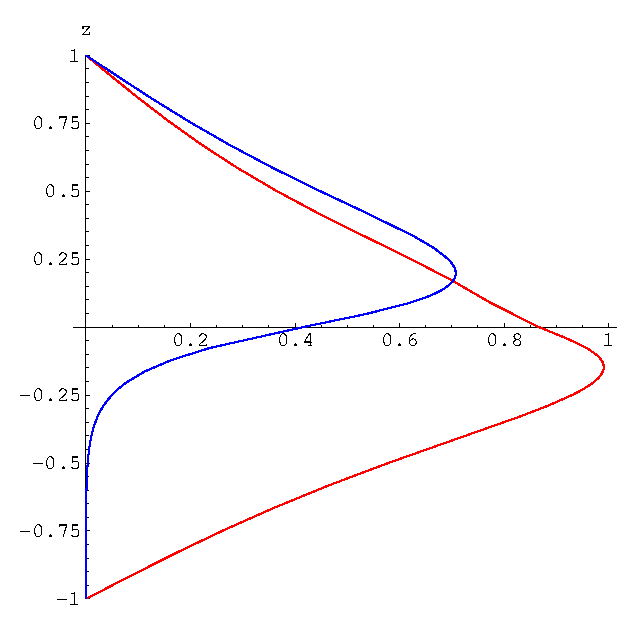
\includegraphics[height=2.5in]{hitplot}}
\put(1.6,.45){$\widehat{\psi}_{r}$}
\put(.5,.8){$\widehat{\psi}_{i}$}
\end{picture}
\end{center}
\caption[Use of {\tt psfrag} system]{This looks ugly until rendered in postscript.
 At that time, the
{\tt z} (which has now vanished) is turned into a $\zeta$.  This will not work
with {\tt pdflatex}.} 
\end{figure}
%%%%%%%%%%%%

\chapter{Other examples}
\label{other}
Note that \LaTeX\ will place Figure \ref{flowchart} after the list,
because I did not use the {\tt [H]} option after the \verb9\begin{figure}9.
\begin{figure}
\begin{center}
\setlength{\unitlength}{1in}
\begin{picture}(4,4)

\put(1.25,3.5){\framebox(1.5,0.5){\shortstack{
control variables}}}

\put(2.,3.4){\vector(0,-1){.25}}
\put(2.1,3.3){\makebox(0,0)[l]{\shortstack{
first estimate of I.C.}}}


\put(1.25,2.5){\framebox(1.5,0.5){\shortstack{
Make forecast using \\ forward model}}}

\put(1.5,2.4){\vector(-1,-1){.25}}
\put(1.3,2.3){\makebox(0,0)[r]{\shortstack{
model output}}}


\put(2.5,2.1){\vector(-1,1){.25}}
\put(2.5,2.2){\makebox(0,0)[l]{\shortstack{
new estimate of I.C.}}}

\put(.25,1.5){\framebox(1.5,.5){\shortstack{
compute \\ cost function J}}}
\put(1.5,1.4){\vector(0,-1){.25}}
\put(-.0,1.75){\vector(1,0){.25}}
\put(-.05,1.75){\makebox(0,0)[r]{\shortstack{
observations}}}


\put(2.25,1.5){\framebox(1.5,.5){\shortstack{
Minimization \\ procedure}}}
\put(2.5,1.1){\vector(0,1){.25}}


\put(.25,.25){\framebox(1.5,.75){\shortstack{
compute \\ Lagrangian \\ multipliers}}}

\put(1.9,.5){\vector(1,0){.25}}

\put(2.25,.25){\framebox(1.5,.75){\shortstack{
compute gradient\\ $\nabla J(c)$ \\ using adjoint model}}}

%\drawline(0.1,1.8)(0.5,1.8)
%\drawline(0.5,1.8)(0.9,3.0)
\end{picture}




\caption[A flowchart]
{Flowchart of data assimilation using the adjoint method.}
\label{flowchart}
\end{center}
\end{figure}

\begin{description}
\item[Step 1:] Make a first estimate of the initial condition (I.C.).
\item[Step 2:] Run the forward model to generate a forecast over the 
assimilation interval.
\item[Step 3:] Compute the cost function, J, using the observations 
and the model output.
\item[Step 4:] Compute the gradient of the cost function with respect 
to the control variable, $\nabla J(c)$, by integrating the adjoint 
model (which is a combination of the forward model and cost 
functional) backwards using the Lagrangian multiplier method.
\item[Step 5:] Generate a new estimate of the initial condition 
(I.C.) for another forecast using a minimization procedure ({\it 
e.g.}, Steepest Descent or Conjugate Gradient Method).  This is done 
iteratively toward the minimum of the cost function using the 
calculated cost function and its gradient.
\item[Step 6:] The process is repeated until some convergence criteria 
are met, {\it i.e.}, the cost functional, J, is near its local minimum.  In 
practice, this is determined by an insignificant change in the 
gradient from one iteration to the next.  If not, the process will be 
terminated when some maximum number of iterations have been achieved.
\end{description}
\section{A Bargraph}
Hey, where did that bargraph go?  I thought I put it in this section!
\label{bargraph}
\begin{figure}
\begin{center}
\centering
\fbox{{\bf Best dense, row-wise algorithms}} \\
\vspace{.5in}
\textbf{Algorithm 1, p=2, gaxpy}\\[5mm]
\begin{barenv}
\setstretch{.3}
\setyaxis{0}{500}{100}\setyname{secs}
\bar{.903}{1}[\texttt{s}]
\bar{116.}{6}[\texttt{1}]
\bar{116.}{1}[\texttt{1}]
\bar{117.}{6}[\texttt{2}]
\bar{58.}{1}[\texttt{2}]
\bar{233.}{6}[\texttt{4}]
\bar{58.}{1}[\texttt{4}]
\bar{465.}{6}[\texttt{8}]
\bar{58.}{1}[\texttt{8}]
\end{barenv}
\caption[CPU Time]{CPU time (hatched) and wall clock time (white) 
for srowdg (s) and a1rowdg with various 
numbers of processors. m=128 N=64}
\label{a1rowdg}
\end{center}
\end{figure}

\section{Some tables}
\label{table}
\begin{table}
\begin{center}
\begin{tabular}{|c|c|} \hline
	time (hours)   &       T (C) \\ \hline
  				   0           &             17.0\\
				   1.5         &            18.8\\
				   3.0         &            19.8\\
				   4.5         &            20.5\\
				   6.0         &            21.0\\
				   7.5         &            21.3\\
				   9.0         &            21.5\\
				  10.5         &           21.8\\
				  12.0         &           22.2\\
				  13.5         &           22.8\\
				  15.0         &           23.5\\
				  16.5         &           24.1\\
				  18.0         &           24.3\\ \hline

\end{tabular}
\caption{T(t) for the initial 18 hours}\label{Tinit}
\end{center}
\end{table}

I will put some text here just to see what happens to it.
 
\begin{table}
\begin{center}
\begin{tabular}{|l|l|l|l|} \hline
Step 1 & \multicolumn{3}{c|}{Step 2} \\ \hline
 & Stage 1 & Stage 2 & Stage 3  \\ \hline
$x_{1}$ & & & \\
$x_{1:2}$ & & & \\
$x_{1:3}$ & & &  \\
$x_{1:4}$ & & & \\ \hline
$x_{5}$ &$x_{1:5}$ & &  \\
$x_{5:6}$,\ $A_{5:6}$ & $x_{1:6}$ & & \\
$x_{5:7}$,\ $A_{5:7}$ & $x_{1:7}$ & &  \\
$x_{5:8}$,\ $A_{5:8}$ & $x_{1:8}$ &&\\ \hline
$x_{9}$& & $x_{1:9}$& \\
$x_{9:10}$,\ $A_{9:10}$ && $x_{1:10}$&  \\
$x_{9:11}$,\ $A_{9:11}$ && $x_{1:11}$ & \\
$x_{9:12}$,\ $A_{9:12}$ &&  $x_{1:12}$ &\\ \hline
$x_{13}$ &&& $x_{1:13}$ \\
$x_{13:14}$,\ $A_{13:14}$ & &&  $x_{1:14}$ \\
$x_{13:15}$,\ $A_{13:15}$ & &&  $x_{1:15}$ \\
$x_{13:16}$,\ $A_{13:16}$ & &&  $x_{1:16}$ \\ \hline
\end{tabular}
\caption[Algorithm \# 3 example]{Algorithm \# 3 example}\label{algo3ex}

\end{center}
\end{table}

\section{Some complicated equations}
To this end, the Lagrangian is introduced
(see \citet{Lanczos} for the theoretical foundations of 
minimizing functions subject to a constraint).
\bea
L(c,\lambda,\mu,\eta) &=& J(c)  \nonumber \\*
&& + \sum_{i=1}^{n}
\lambda_{i}\left[
\theta_{i}-\theta_{i-1}
-\frac{\tau}{h_{i-1}}C_{T}V(1+K)
\left(T_{i-1} - \theta_{i-1} \right)
\right] \nonumber \\*
&& + \sum_{i=1}^{n}
\mu_{i}\left[
h_{i}-h_{i-1}
-\tau K C_{T}V
\frac{\left(T_{i-1} - \theta_{i-1} \right)}
{\sigma_{i-1}}
-\tau W
\right]  \nonumber \\*
&& + \sum_{i=1}^{n}
\eta_{i}\left[
\sigma_{i}-\sigma_{i-1}
+\frac{\tau}{h_{i-1}}C_{T}V(1+K)
\left( T_{i-1} - \theta_{i-1} \right) \right.
\nonumber \\*
&&
\left. \qquad -\tau \gamma K C_{T}V
\frac{\left(T_{i-1} - \theta_{i-1} \right)}
{\sigma_{i-1}}
-\tau \gamma W
\right]
\label{niceeq}
\eea
where $\lambda=\left(\lambda_{1},\ldots,\lambda_{n}\right)^{t}$,
$\mu=\left(\mu_{1},\ldots,\mu_{n}\right)^{t}$,
$\eta=\left(\eta_{1},\ldots,\eta_{n}\right)^{t}$
are the undetermined Lagrangian 
multipliers in (\ref{niceeq}).   

\be
E=
\left[
\begin{array}{cccccccc}
-I_{3} & 0 & 0 & 0 & \ldots & 0 & 0 &0 \\
D_{1} & -I_{3} & 0 & 0 & \ldots & 0 & 0 &0 \\
0 & D_{2} & -I_{3}  & 0 & \ldots & 0 & 0 &0 \\
\ldots & \ldots & \ldots  & \ldots & \ldots & \ldots & \ldots &\ldots \\
0 & \ldots & \ldots  & \ldots & \ldots & \ldots & D_{n-1} & -I_{3} \\
\end{array}
\right],
\label{Edef}
\ee

By definition,
\bea
\epsilon_{i}^{\theta} &=& \theta_{i} - \overline{\theta}_{i},\label{one}\\* 
\epsilon_{i}^{h} &=& h_{i} - \overline{h}_{i},\label{two}  \\* 
\epsilon_{i}^{\sigma} &=& \sigma_{i} - \overline{\sigma}_{i}. 
\label{three} 
\eea
Now we can still refer to (\ref{Edef}) or (\ref{one})-(\ref{three}).

%
%\references{agsm}{myreferences}
\references{amermeteorsoc}{myreferences}
%comment out the next four lines if you don't have an appendix
\appendix
\chapter{A Long Proof}
\OUdoublespace
%%%%%following needed for Appendix, appex.tex
\renewcommand{\th}{\theta} %\th is defined as an obscure character called a "thorn",
                           %so we must use renewcommand to override it
\newcommand{\thl}{\th_l}  %these commands are undefined by default, so use newcommand
\newcommand{\p}[1]{\left( #1 \right)}
\newcommand{\sqrb}[1]{\left[ #1 \right]}
\renewcommand{\b}[1]{\overline{#1}}
\newcommand{\thv}{\th_v}
\newcommand{\Lcp}{\frac{L}{c_p}}
\newcommand{\fth}{\b{w'\th'}}
\newcommand{\fthl}{\b{w'\thl'}}
\newcommand{\fthv}{\b{w'\thv'}}
\newcommand{\fqt}{\b{w'q_t'}}
\newcommand{\fqs}{\b{w'q_s'}}
\newcommand{\fqv}{\b{w'q_v'}}
%%%
The buoyancy production term requires a closure for $\fthv$.  In saturated
conditions $q_l=q_s$ and we have 3 linear relations between 5 flux densities:
\bea
\fth &=& \fthl + B\fqt -B\fqs \label{feq1}\\
\fthv &=& C\fth + D\fqs -E\fqt \label{feq2}\\
\fqs &=& F\fth \label{feq3}
\eea
where
\bea
B &\equiv& \chi \Lcp \\
C &\equiv& 1 + 1.61 \b{q_s} - \b{q_t}\\
D &\equiv& 1.61 \b{\th}\\
E &\equiv& -\b{\th}\\
F &\equiv& 0.622 \frac{L \b{q_s}}{R_d \b{T} \b{\th}} 
\eea
We will eliminate $\fqs$ and $\fth$ from (\ref{feq1})-(\ref{feq3}) and
thus derive a linear relation between $\fthv$ and $\fthl$ and $\fqt$:
\be
\fthv = \frac{C+DF}{1+BF}\fth + \p{\frac{C+D F}{1+BF}B -E}\fqt 
\ee
Eq. (\ref{feq3}) has been derived from the Clausius-Clapyron equation
\be
\frac{d e_s}{d T}=e_s \frac{L}{R_dT^2}
\ee
and
\be
q_s \equiv 0.622\frac{e_s}{p}
\ee
followed by assumptions that $p'\over \b{p}$ is small compared with both
$\frac{1}{e_s}\frac{de_s}{dT}T'$ and $T' \over \b{T}$.
Here is how we calculate $\lambda$:
\be
e(z)= \int_z^{z+\lambda_{up}(z)} \frac{g}{\b{\thv}(z')} \sqrb{ \b{\thv}(z) - \b{\thv^*}(z')}dz'
\ee
\be
e(z)= \int_z^{z-\lambda_{down}(z)} \frac{g}{\b{\thv}(z')} \sqrb{ \b{\thv}(z) - \b{\thv^*}(z')}dz'
\ee
\be
\lambda(z)=\sqrb{ \lambda_{down}(z) \lambda_{up}(z) }^{1/2}
\ee

\end{document}
